% paper template

\documentclass[10pt,reqno,final]{amsart}
%\documentclass[10pt,reqno,draft]{amsart}

% package for mathematics
\usepackage{amsmath,amssymb,amsthm}
% package for RSFS fonts in maths
\usepackage{mathrsfs}
% package for special symbols
\usepackage{pifont}
% package for multilingual support
\usepackage[english]{babel}
% package for figures
\usepackage{graphicx}
\usepackage{subfig}
% package for hyperlink
\usepackage{hyperref}
% package for layout of list
\usepackage{enumitem}
% package for showing keys in draft mode
\usepackage[notcite,notref]{showkeys}
% package for color
\usepackage{color}
% package for table
\usepackage{tabularx}
\usepackage{booktabs}
\usepackage{array}
\usepackage{makecell}
% package for multiple columns and rows
\usepackage{multirow,multicol}
% package for caption
\usepackage{caption}
% package for algorithm
\usepackage{algorithm,algorithmicx}
\usepackage{algpseudocode}
% package for using box and verbatim
\usepackage{fancybox}
% package for address
\usepackage[foot]{amsaddr}

% hyperlink setting
%\hypersetup{
%  colorlinks=true,
%  linkcolor=magenta,
%  citecolor=blue,
%  filecolor=blue,
%  urlcolor=blue
%}

% package for bibliography support
\usepackage{cite}
%\usepackage[numbers,sort&compress]{natbib}

% allow page breaks between multiline formulas
\allowdisplaybreaks

% layout setting
\usepackage{geometry}
\geometry{left=1.25in,right=1.25in,top=1.25in,bottom=1.25in}
%\setlength{\textwidth}{15cm}
%\setlength{\textheight}{21.6cm}
%\setlength{\oddsidemargin}{0.5cm}
%\setlength{\evensidemargin}{0.5cm}

% command for line spacing
\renewcommand{\baselinestretch}{1.1}

% command for mark footnotes
%\usepackage[symbol]{footmisc}
%\renewcommand{\thefootnote}{\fnsymbol{footnote}}

% command for equations, theorems and lemmas etc.
\theoremstyle{plain}
\newtheorem{theorem}{Theorem}[section]
\newtheorem{lemma}{Lemma}[section]
\newtheorem{corollary}{Corollary}[section]

\theoremstyle{definition}
\newtheorem{definition}{Definition}[section]
\newtheorem{example}{Example}
\newtheorem{xca}{Exercise}[section]

\theoremstyle{remark}
\newtheorem{remark}{Remark}[section]

% caption setting
%\captionsetup{font={small,singlespacing},labelformat={default},labelsep=period}
\captionsetup[figure]{position=bottom,skip={8pt},name={Figure}}
\captionsetup[table]{position=top,skip={4pt},name={Table}}
%\setlength{\textfloatsep}{12pt plus 2pt minus 2pt}
%\setlength{\floatsep}{10pt plus 2pt minus 2pt}
%\setlength{\intextsep}{10pt plus 2pt minus 2pt}
%\setlength{\abovecaptionskip}{2pt plus 1pt minus 1pt}
%\setlength{\belowcaptionskip}{3pt plus 1pt minus 2pt}

% number of equation, figure and table
\numberwithin{equation}{section}
\numberwithin{figure}{section}
\numberwithin{table}{section}

% graphic path
\graphicspath{{./figures/}}

% blank box for figure
\newcommand{\blankbox}[2]{%
  \parbox{\columnwidth}{\centering
  \setlength{\fboxsep}{0pt}%
  \fbox{\raisebox{0pt}[#2]{\hspace{#1}}}}%
}

% differential operator
\newcommand{\dif}{\mathop{}\!\mathrm{d}}

% new command
\newcommand{\abs}[1]{\lvert#1\rvert}
\newcommand{\norm}[1]{\lVert#1\rVert}
\newcommand{\dx}[1][x]{\mathop{}\!\mathrm{d}#1}
\newcommand{\ii}{\mathrm{i}\mkern1mu} % imaginary
\newcommand{\refe}[2]{(\ref{#1})--(\ref{#2})}
\newcommand{\red}[1]{\textcolor{red}{#1}}


% Information for title and author
\title[Short Title]{This is Full Title}

\author[Author A]{Author A$^{1}$}
\author[Author B]{Author B$^{2}$}
\author[Author C]{Author C$^{1,*}$}
\address{$^{1}$Common address of authors A and B}
\address{$^{2}$Author C address}

%\author[Author A, Author B]{Author A$^{1}$, Author B$^{1,*}$}
%\address{$^{1}$Common address of authors A and B}
%\author[Author C]{Author C$^{2}$}
%\address{$^{2}$Author C address}

\email{list of emails}

\thanks{${}^{*}$Corresponding author}
\thanks{The first author was supported in part by NSFC Grant \#000000.}
\thanks{Support information for the second author.}
\thanks{Support information for the third author.}

\subjclass[2000]{65M60, 65M12}

\date{\today}

\keywords{Keyword 1, keyword 2, error analysis}


\begin{document}

\begin{abstract}
This is an example \LaTeX\ article. This can be used as a template for new articles.
Abstracts must be able to stand alone and so cannot contain citations to the paper's references,equations, etc.
An abstract must consist of a single paragraph and be concise.
Because of online formatting, abstracts must appear as plain as possible.
Any equations should be inline.
\end{abstract}

\maketitle


\section{Introduction}

The introduction introduces the context and summarizes the manuscript.
It is important to clearly state the contributions of this piece of work.

In this paper we present a new method for solving the model equation
\begin{equation}\label{eq:mulequ}
\left\{\begin{aligned}
  & \partial_{t} u-\varepsilon^{2} \Delta u+u^{3}-u=0, \quad \text{in} ~\Omega\times\mathcal{T}, \\
  &\, u(x,y,t) = g(t), \quad \text{on } ~ \partial \Omega, \\
  &\, u(x,y,0)=\varphi(x, y), \quad \text{on } ~\Omega.
\end{aligned}\right.
\end{equation}
where $\varepsilon$ is a small parameter.

This is an example of quoting an equation \eqref{eq:mulequ}.

The merits of our method are as follows:
\begin{itemize}
  \item item one
  \item item two
  %\item item three
\end{itemize}
\begin{enumerate}
  \item item one
  \item item two
  %\item item three
\end{enumerate}

The outline is not required, but we show an example here.

The paper is organized as follows. Our main results are in \ref{sec:main},
our new algorithm is in \ref{sec:alg}, experimental results are in \ref{sec:experiments},
discussion is in \ref{sec:discussion} and the conclusions follow in \ref{sec:conclusions}.


\section{Preliminaries}
\label{sec:preliminaries}

\subsection{This is subsection}

\subsubsection{This is subsubsection}


\section{Main results}
\label{sec:main}

We interleave text filler with some example theorems and theorem-like items.

\begin{definition}
This is a definition environment.
\end{definition}

\begin{lemma}
This is a lemma environment.
\end{lemma}

\begin{theorem}
This is a theorem environment.
\end{theorem}
\begin{proof}
  This is a proof environment.
\end{proof}

\begin{lemma}
This is a lemma environment
\begin{enumerate}[label=\rm (\roman*)]
  \item item A
  \item item B
  \begin{equation}\label{eq:limite}
    \lim_{n\to\infty}\left(1+\frac{1}{n}\right)^n=e.
  \end{equation}
\end{enumerate}
\end{lemma}

This is a citation example \cite{Adams2003,TreWei2014}.
This statement requires citations \cite{Shen1994,Tadmor2012,TreWei2014}.

Here we state our main result as \ref{thm:bigthm}.

\begin{theorem}[$LDL^T$ Factorization \cite{GoVa2013}]\label{thm:bigthm}
  If $A \in \mathbb{R}^{n \times n}$ is symmetric and the principal submatrix $A(1:k,1:k)$ is nonsingular for $k=1:n-1$, then there
  exists a unit lower triangular matrix $L$ and a diagonal matrix
  \begin{equation*}
    D = \operatorname{diag}(d_1,\dots,d_n),  %\diag(d_1,\dots,d_n)
  \end{equation*}
  such that $A=LDL^T$. The factorization is unique.
\end{theorem}

%LaTeX is a high-quality typesetting system; it includes features designed
%for the production of technical and scientific documentation.

\begin{theorem}[Mean Value Theorem]\label{thm:mvt}
  Suppose $f$ is a function that is continuous on the closed interval $[a,b]$ and differentiable on the open interval $(a,b)$.
  Then there exists a number $c$ such that $a < c < b$ and
  \begin{equation*}
    f'(c) = \frac{f(b)-f(a)}{b-a}.
  \end{equation*}
  In other words,
  \begin{equation*}
    f(b)-f(a) = f'(c)(b-a).
  \end{equation*}
\end{theorem}

\begin{remark}
Observe that \ref{thm:bigthm}, \ref{thm:mvt} correctly mix references to multiple labels.
\end{remark}

% command cref package cleveref
%Observe that \cref{thm:bigthm,thm:mvt,cor:a} correctly mix references
%to multiple labels.

\begin{corollary}\label{cor:a}
  Let $f(x)$ be continuous and differentiable everywhere.
  If $f(x)$ has at least two roots, then $f'(x)$ must have at least one root.
\end{corollary}
\begin{proof}
  Let $a$ and $b$ be two distinct roots of $f$.
  By \ref{thm:mvt}, there exists a number $c$ such that
  \begin{equation*}
    f'(c) = \frac{f(b)-f(a)}{b-a} = \frac{0-0}{b-a} = 0.
  \end{equation*}
\end{proof}

Note that it may require two \LaTeX\ compilations for the proof marks to show.

Display matrices can be rendered using environments from \texttt{amsmath}:
\begin{equation}\label{eq:matrices}
S=\begin{bmatrix}1&0\\0&0\end{bmatrix}
\quad\text{and}\quad
C=\begin{pmatrix}1&1&0\\1&1&0\\0&0&0\end{pmatrix}.
\end{equation}
Equation \ref{eq:matrices} shows some example matrices.

We calculate the Fr\'{e}chet derivative of $F$ as follows:
\begin{subequations}
\begin{align}
  F'(U,V)(H,K)
  &= \langle R(U,V),H\Sigma V^{T} + U\Sigma K^{T} -
  P(H\Sigma V^{T} + U\Sigma K^{T})\rangle \label{eq:aa} \\
  &= \langle R(U,V),H\Sigma V^{T} + U\Sigma K^{T}\rangle
  \nonumber \\
  &= \langle R(U,V)V\Sigma^{T},H\rangle +
  \langle \Sigma^{T}U^{T}R(U,V),K^{T}\rangle. \label{eq:bb}
\end{align}
\end{subequations}
\ref{eq:aa} is the first line, and \ref{eq:bb} is the last line.


\section{Algorithm}
\label{sec:alg}

Our analysis leads to the algorithm in \ref{alg:buildtree}.

\begin{algorithm}
\caption{Build tree}
\label{alg:buildtree}
\begin{algorithmic}
  \State {Define $P:=T:=\{ \{1\},\ldots,\{d\}$\}}
  \While{$\#P > 1$}
    \State {Choose $C^\prime\in\mathcal{C}_p(P)$ with $C^\prime := \operatorname{argmin}_{C\in\mathcal{C}_p(P)} \varrho(C)$}
    \State {Find an optimal partition tree $T_{C^\prime}$ }
    \State {Update $P := (P{\setminus} C^\prime) \cup \{ \bigcup_{t\in C^\prime} t \}$}
    \State {Update $T := T \cup \{ \bigcup_{t\in\tau} t : \tau\in T_{C^\prime}{\setminus} \mathcal{L}(T_{C^\prime})\}$}
  \EndWhile
  \State \Return $T$
\end{algorithmic}
\end{algorithm}

Adjust the width of the algorithm environment
\begin{center}
\vspace{-2ex}
\begin{minipage}{0.9\linewidth}
\begin{algorithm}[H]
\caption{Euclid’s algorithm}
\label{alg:euclid}
\begin{algorithmic}[1] % line numbering
\Procedure{Euclid}{$a,b$}\Comment{The g.c.d. of a and b}
  \State $r \gets a \bmod b$
  \While{$r\not=0$}\Comment{We have the answer if r is 0}
    \State $a \gets b$
    \State $b \gets r$
    \State $r \gets a \bmod b$
  \EndWhile\label{euclidendwhile}
  \State \textbf{return} $b$\Comment{The gcd is b}
\EndProcedure
\end{algorithmic}
\end{algorithm}
\end{minipage}
\end{center}


\section{Experimental results}
\label{sec:experiments}

Some experimental results here.

\begin{example}
  This is example environment.
\end{example}

\begin{figure}[htp!]
\blankbox{.6\columnwidth}{10pc}
\caption{This is an example of a figure caption with text.}
\label{fig:blackbox}
\end{figure}

\clearpage
\textbf{Some figures and tables here.}

Figure~\ref{fig:foo} shows some example results.
\begin{figure}[htp!]
  \centering
  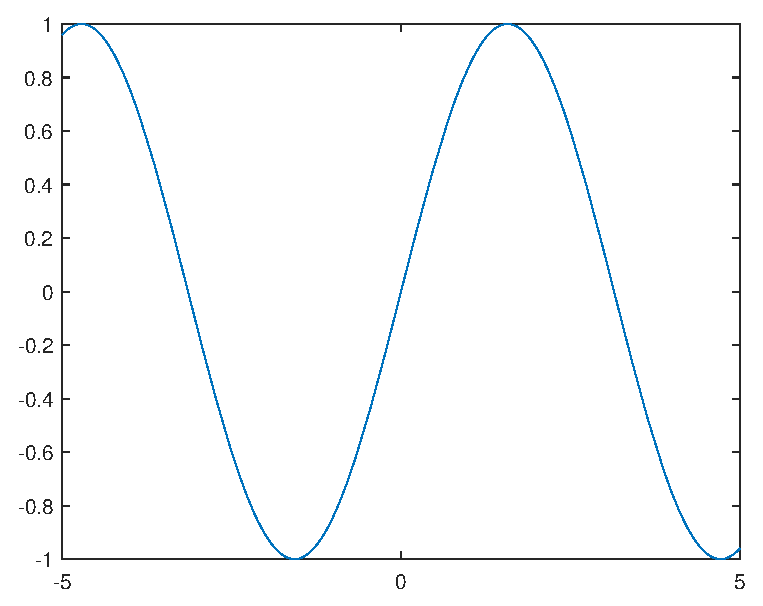
\includegraphics[width=0.48\linewidth]{fig1}
  \caption{Example figure using external image files.}
  \label{fig:foo}
\end{figure}

The two figures are placed side by side, sharing one title, as shown in \autoref{fig:twofigs}.
\begin{figure}[htp!]
  \centering
  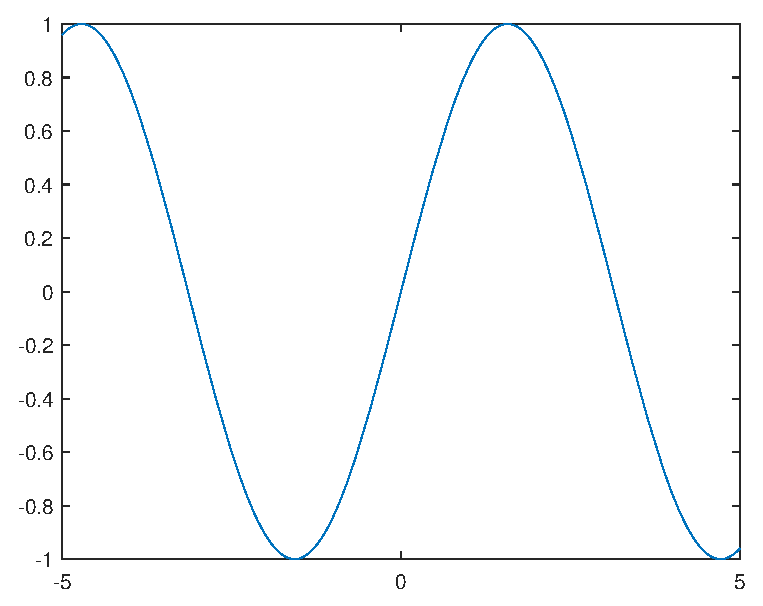
\includegraphics[width=0.45\linewidth]{fig1}
  \hfill
  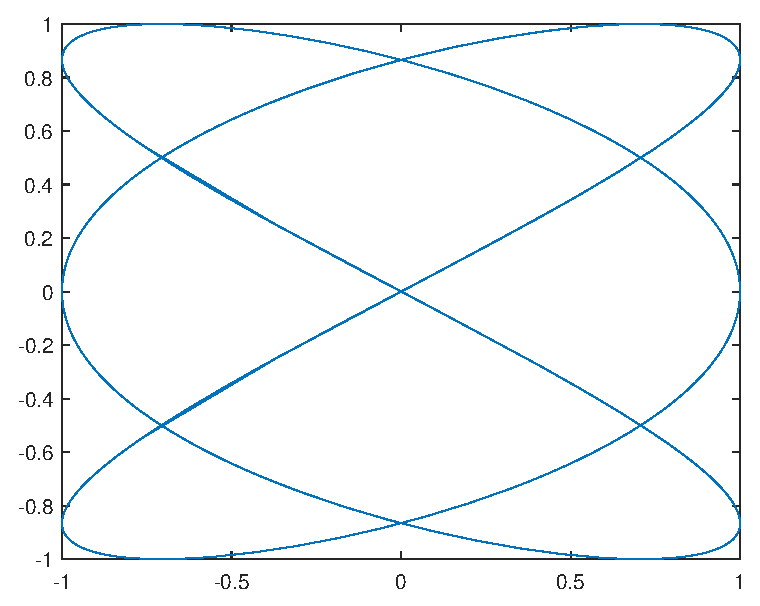
\includegraphics[width=0.45\linewidth]{fig2}
  \caption{Left: Caption 1, Right: Caption 2.}
  \label{fig:twofigs}
\end{figure}

Use the \texttt{tabularx} environment to generate \autoref{tab:error}. 
The defined column type \texttt{P} also works for \texttt{tabular} environment.

\begin{table}[htp!]
\centering
\newcolumntype{L}{X}
\newcolumntype{C}{>{\centering \arraybackslash}X}
\newcolumntype{R}{>{\raggedleft \arraybackslash}X}
\newcolumntype{P}[1]{>{\centering \arraybackslash}p{#1}}
\renewcommand\arraystretch{1.2}
\caption{Table description}
\label{tab:error}
\begin{tabularx}{0.8\textwidth}{|P{0.8cm}|C|C|C|C|C|}
\Xhline{2\arrayrulewidth}
N  & A       & B    & C       & D      & E     \\
\Xhline{2\arrayrulewidth}
2  & 9.20E-05 & 9.90E-05 & 1.00E-06 & 8.00E-06 & 1.50E-05 \\
4  & 9.80E-05 & 8.00E-05 & 7.00E-06 & 1.40E-05 & 1.60E-05 \\
6  & 4.00E-06 & 8.10E-05 & 8.80E-05 & 2.00E-05 & 2.20E-05 \\
8  & 8.50E-05 & 8.70E-05 & 1.90E-05 & 2.10E-05 & 3.00E-06 \\
10 & 8.60E-05 & 9.30E-05 & 2.50E-05 & 2.00E-06 & 9.00E-06 \\
12 & 1.70E-05 & 2.40E-05 & 7.60E-05 & 8.30E-05 & 9.00E-05 \\
%14 & 2.30E-05 & 5.00E-06 & 8.20E-05 & 8.90E-05 & 9.10E-05 \\
%16 & 7.90E-05 & 6.00E-06 & 1.30E-05 & 9.50E-05 & 9.70E-05 \\
\Xhline{2\arrayrulewidth}
\end{tabularx}
\end{table}

Some description and explanation of pictures and tables.

Use \texttt{minipage} package to set images side-by-side, each with its own title,
as shown in Figure~\ref{fig:A} and Figure~\ref{fig:B}.

\begin{figure}[htp!]
\begin{minipage}[t]{0.48\linewidth}
  \centering
  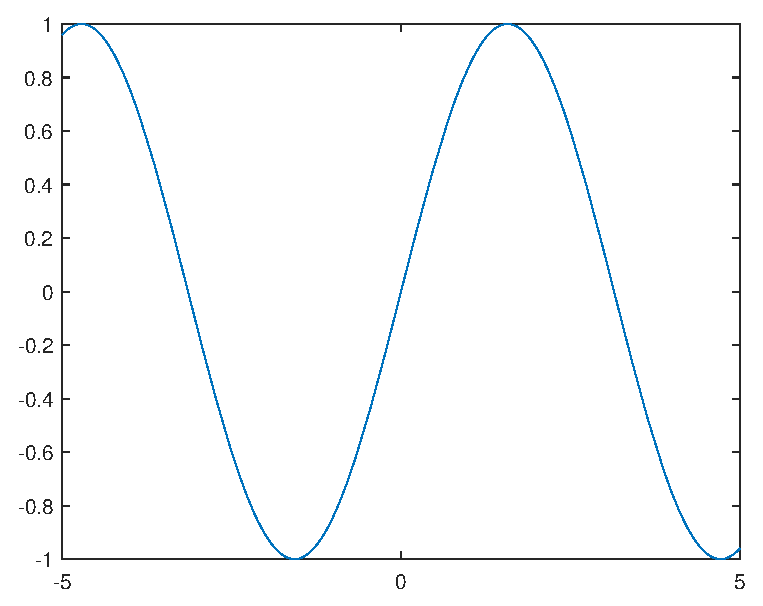
\includegraphics[width=0.96\linewidth]{fig1}
  \caption{Caption A}
  \label{fig:A}
\end{minipage}
\hfill
\begin{minipage}[t]{0.48\linewidth}
\centering
   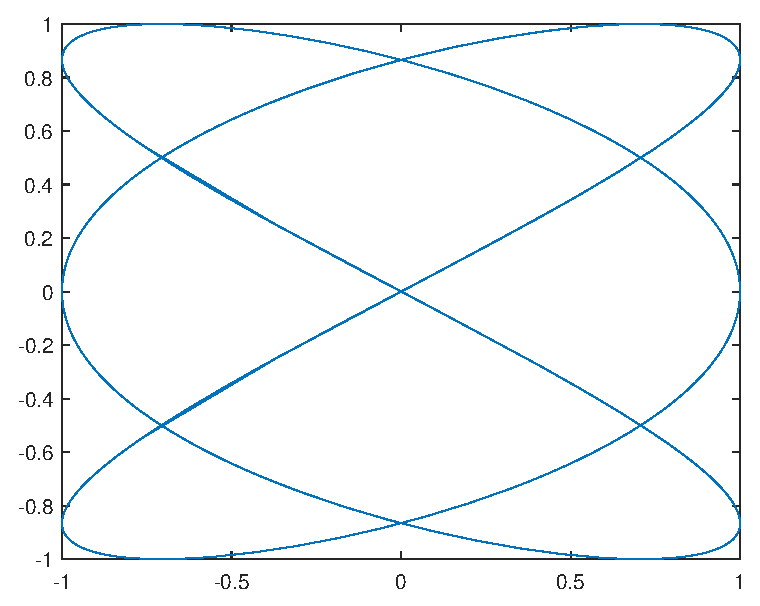
\includegraphics[width=0.96\linewidth]{fig2}
   \caption{Caption B}
   \label{fig:B}
\end{minipage}
\end{figure}

Use \texttt{subfig} package to set subfigure, each with its subcaption, as shown in Figure~\ref{fig:twosubfig}.

\begin{figure}[htp!]
\centering
\subfloat[Subcaption A]{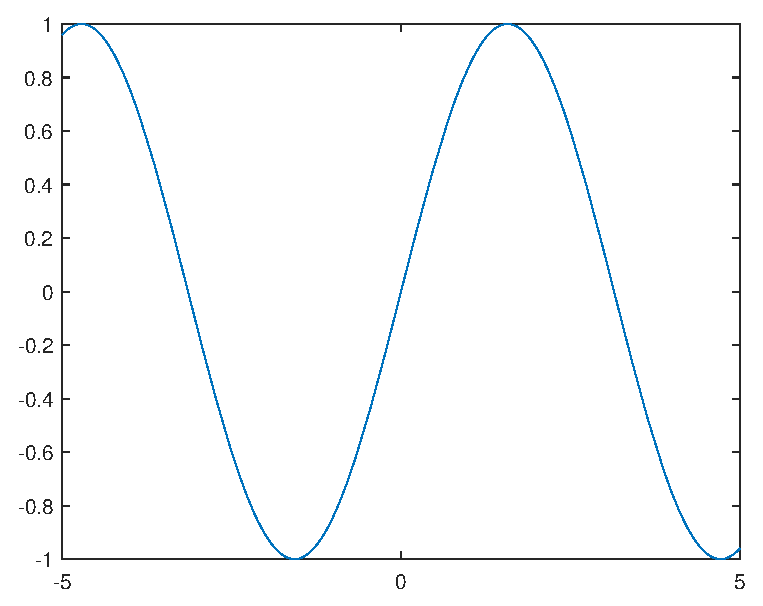
\includegraphics[width=0.46\linewidth]{fig1}}
\qquad
\subfloat[Subcaption B]{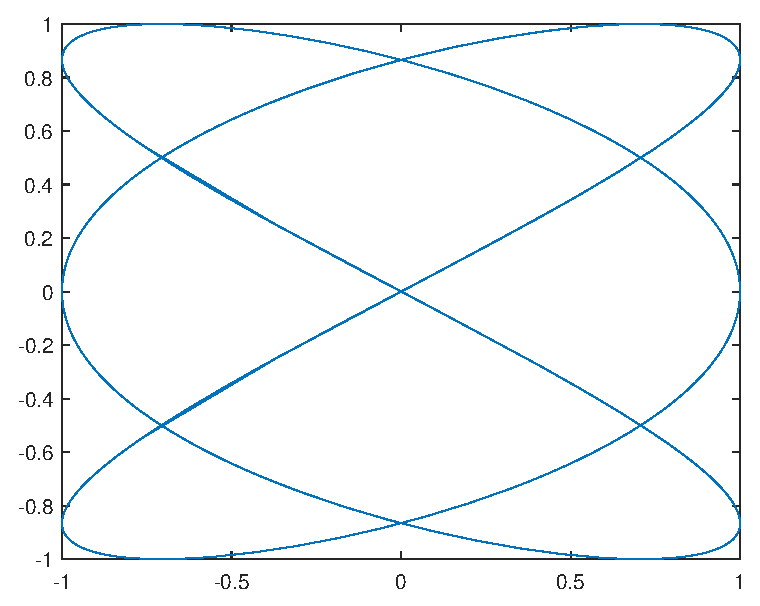
\includegraphics[width=0.46\linewidth]{fig2}}
\caption{Two subfigures}
\label{fig:twosubfig}
\end{figure}

Additional results are available in the supplement in Table~\ref{tab:foo}.

\begin{table}[!htp]
\centering
\renewcommand\arraystretch{1.2} % line spacing
\caption{Numerical error}
\label{tab:foo}
\begin{tabular}{c|c|cc|cc|cc}
\hline
degree & step-size~$h$ & $L^2$-errors & order & $H^1$-errors & order & $L^\infty$-errors & order \\
\hline
  & 1/128 & 9.18E-06 & 2.02 & 7.70E-03 & 1.01 & 6.46E-07 & 2.02 \\
1 & 1/256 & 2.29E-06 & 2.01 & 1.92E-03 & 1.00 & 1.61E-07 & 2.01 \\
  & 1/512 & 5.70E-07 & 2.00 & 9.56E-04 & 1.00 & 4.01E-08 & 2.00 \\
\hline  % \cline{1-8}
  & 1/128 & 1.39E-08 & 3.01 & 1.15E-05 & 2.01 & 3.48E-12 & 4.02 \\
2 & 1/256 & 1.73E-09 & 3.01 & 2.88E-06 & 2.01 & 3.27E-13 & 3.94 \\
  & 1/512 & 2.17E-10 & 3.00 & 7.24E-06 & 2.00 & 6.66E-13 & 1.55 \\
\hline  % \cline{1-8}
  & 1/32  & 2.28E-09 & 4.05 & 6.92E-07 & 3.04 & 1.45E-15 & 8.21 \\
3 & 1/64  & 1.42E-10 & 4.03 & 8.65E-08 & 3.02 & 2.06E-14 & 3.85 \\
  & 1/128 & 8.91E-12 & 4.01 & 1.08E-08 & 3.01 & 3.86E-14 & 0.91 \\
\hline
\end{tabular}
\end{table}


\section{Discussion of \texorpdfstring{{$Z=X \cup Y$}}{Z = X union Y}}
\label{sec:discussion}

Some discussions here. Some discussions here. Some discussions here.
Some discussions here. Some discussions here. Some discussions here.
Some discussions here. Some discussions here.

Some discussions here. Some discussions here. Some discussions here.
Some discussions here. Some discussions here. Some discussions here.
Some discussions here. Some discussions here.

\section{Conclusions}\label{sec:conclusions}

Some conclusions here. Some conclusions here. Some conclusions here.
Some conclusions here. Some conclusions here. Some conclusions here.
Some conclusions here.

Some conclusions here. Some conclusions here. Some conclusions here.
Some conclusions here. Some conclusions here. Some conclusions here.
Some conclusions here. Some conclusions here.


\appendix
\section{An example appendix}

The contents of the appendix are here.

\begin{lemma}
Test Lemma.
\end{lemma}

This is a equation in appendix.
\begin{equation}\label{eq:abc}
  a^2+b^2=c^2.
\end{equation}

\section*{Acknowledgments}

We would like to acknowledge the assistance of volunteers in putting together this example manuscript and supplement.


% References
\bibliographystyle{plain}
%\bibliographystyle{abbrv}
%\bibliographystyle{amsplain}

\bibliography{reference}


\end{document}

